\chapter{MULTIPLE OBJECT TRACKING}

\renewcommand{\headrulewidth}{0.5pt}
\renewcommand{\footrulewidth}{0.5pt}
\thispagestyle{plain}
\pagestyle{fancy}
\fancyhf{}
\fancyhead[L]{\textbf{CHAPTER 3}}
\fancyhead[R]{\textbf{Intelligent Traffic System}}
\raggedright
\fancyfoot[L]{From: ITM Vision}
\fancyfoot[R]{Page \thepage}

\section{Overview}
    Multiple object tracking can be viewed as a multi-variable estimation problem. Given an image sequence, we employ
    $s_t^i$ to denote the state of the i-th object in the t-th frame, $\textbf{S}_t = (s_t^1, s_t^2, ..., s_t^{M_t})$
    to denote states of all the $M_t$ objects in the t-th frame. Let \textbf{$s_{i_s:i_c}^i = \{s_{i_s}^i,...,s_{i_e}^i\}$} 
    be the sequential states of the i-th object, where $i_s$ and $i_e$ are respectively the first and last frame in 
    which target \emph{i} exist, and \textbf{$S_{1:t} = \{S_1,S_2,...,S_t\}$} to denote all the sequential states of all the 
    objects from the first frame to the t-th frame. Note that the object number may vary from frame to frame. \\ 
    \vspace{3mm}
    Correspondingly, following the most commonly used tracking by detection, or Detection Based Tracking (DBT) paradigm,
    we utilize $o_t^i$ to denote the collected observations for the i-th object in the t-th frame. $\textbf{O}_t=(\textbf{o}_t^1,\textbf{o}_t^2,...,\textbf{o}_t^{M_t})$ 
    to denote the collected observations for all the $M_t$ objects in the t-th frame, and $\textbf{O}_{1:t}=\{\textbf{O}_1,\textbf{O}_2,...,\textbf{O}_t\}$ 
    to denote all collected sequential observations of all the objects from the first frame to the t-th frame.
    \vspace{3mm}
    The objective of multiple object tracking is to find the “optimal” sequential states of all the objects, which can be 
    generally modeled by performing MAP (maximal a posteriori) estimation from the conditional distribution of the 
    sequential states given all the observations: 
    \begin{align}
        \hat{S}_{1:t}=\underset{S_{1:t}}{argmax}P(\textbf{S}_{1:t}|\textbf{O}_{1:t})
    \end{align} 
    Different MOT algorithms from previous works can now be thought as designing different approaches to solving 
    the above MAP problem, either from a probabilistic inference perspective or a deterministic optimization perspective. 

\section{Categorization}
    Categorization of MOT bases on: initialization method, processing mode and type of output.
    \begin{itemize}
        \item Initialization method: MOT devides into detection based tracking and detection free tracking
            \begin{itemize}
                \item Detection based tracking: Given a sequence, type specific object detection or motion detection (based on background modeling) is applied in each frame 
                to obtain object hypotheses, then (sequential or batch) tracking is conducted to link detection hypotheses into trajectories. Detection based tracking focuses 
                on specific objects and its performance relies heavily on accuracy of object detectors. Detection based tracking is more popular as it can deal with new 
                discovered and disappear objects automatically.
                \item Detection free tracking requires requires manual initialization of objects in each frame.
                    \begin{figure}[H]
                        \centering
                        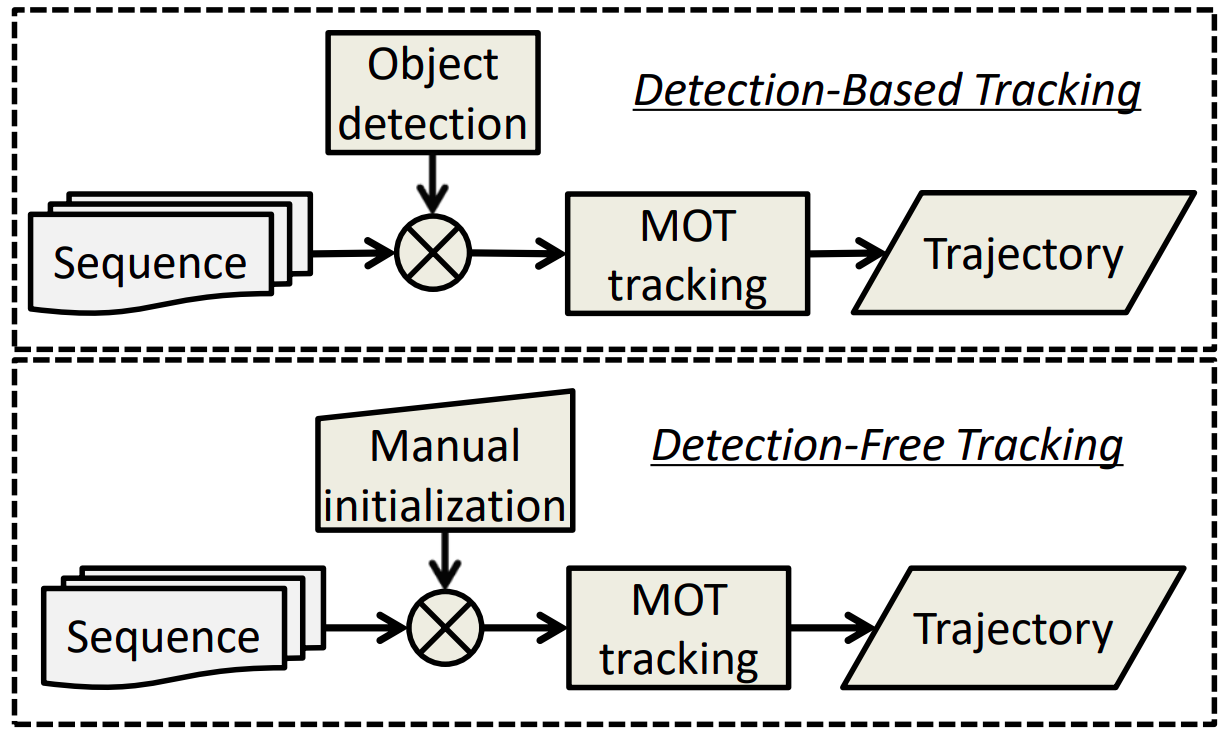
\includegraphics[width=0.6\linewidth]{img/MOT.png}
                        \caption{Pipeline of detection based tracking and detection free tracking}
                    \end{figure}
            \end{itemize}
        \item Processing mode: based on processing mode, MOT can be divided into online tracking and offline tracking problem. 
            \begin{itemize}
                \item An online model receives video input on a frame-by-frame basis, and has to give an output for each frame. This means that, in addition to the current frame, 
                only information from past frames can be used. Online tracking takes up-to-time observation and updates trajectories on the fly there for it is suitable for real time application.
                \item Offline models, on the other hand, have access to the entire video, which means that information from both past and future frames can be used. The task can then be viewed as an 
                optimization problem, where the goal is to find a set of paths that minimize some global loss  function. Offline tracking takes a batch of frames to process therefore it products delay results. 
                Since offline trackers have access to more information, one can expect better performance from these models. 
            \end{itemize}
    \end{itemize}
    Detection free tracking process data sequentially while in Detection based tracking, tracklet or detection response are often associated in batch. \\ 
    \vspace{3mm}
    Recently with the rise of deep learning, MOT can also devided into non-deep learning based methods and deep learning based methods. \\ 
    \vspace{3mm}
    In deep learning based methods, first CNN-based object detectors are applied such as Faster R-CNN and YOLOv3 to localize all objects of interest in input images. Then in a separate step,they crop the images 
    according to the boxes and feed them to an identity embedding network to extract re-ID features which are used to link the boxes over time. The linking step usually follows a standard practice which first 
    computes a cost matrix according to the re-ID features and Intersection over Unions (IoU) of the bounding boxes and then uses the Kalman Filter and Hungarian algorithm to accomplish the linking task. 
    MOT methods based on deep learning can be further devided into two-stage method and one-stage method. \\ 
    \vspace{3mm}
    The main advantage of the two-step methods is that they can develop the most suitable model for each task separately without making compromise. In addition, they can crop the image patches according to the 
    detected bounding boxes and resize them to the same size before estimating re-ID features. This helps to handle the scale variations of objects.The main drawback due to the fact that they are usually very 
    slow because the two tasks need to be done separately without sharing. \\ 
    \vspace{3mm}
    For one stage method, the core idea is to simultaneously accomplish object detection and identity embedding (re-ID features) in a single network in order to reduce inference time. However, the accuracy of the 
    one-shot trackers is usually lower than that of the two-step ones.

\section{MOT Components Overview}
    \subsection{Appearance Model}
        Appearance model includes visual representation and statistical measuring. Appearance model is important cue for affinity computation in MO. Visual representation: local features, region features, 
        Probabilistic Occupancy Map (POM), depth features, Statistical measuring: single cue \& multiple cues (five kinds of fusion strategies: Boosting, Concatenating, Summation, Product, and Cascading).
    \subsection{Motion Model}
        Motion model includes linear \& non-linear model. It aims to estimates the potential position of objects in the future frames, thereby reducing the search space.
    \subsection{Interaction Model} 
        Interaction model, also known as mutual motion model, captures the influence of an object on other objects. In the crowd scenery, an object would experience some “force” from other agents and objects. 
        Interaction model includes social force model \& crowd motion pattern model.
    \subsection{Exclusion Model}
        Exclusion model includes detection-level exclusion \& trajectory-level exclusion. Exclusion is a constraint employed to avoid physical collisions when seeking a solution to the MOT problem. It arises from 
        the fact that two distinct objects cannot occupy the same physical space in the real world.
    \subsection{Occlusion Handling}
        Occlusion is perhaps the most critical challenge in MOT. It is a primary cause for ID switches or fragmentation of trajectories. In order to handle occlusion, various kinds of strategies have been proposed such as: 
        part-to-whole, hypothesize-and-test, buffer-and-recover.
    \subsection{Inference Models}
        \begin{itemize}
            \item \textbf{Probabilistic Inference} \\ 
                Approaches based on probabilistic inference typically  represent states of objects as a distribution with uncertainty. The goal of a tracking algorithm is to estimate the probabilistic distribution of target state 
                by a variety of probability reasoning methods based on existing observations. This kind of approach typically requires only the existing, i.e. past and present observations, thus they are especially appropriate for 
                the task of online tracking. \\
                \vspace{3mm}
                Although the probabilistic approaches provide a more intuitive and complete solution to the problem, they are usually difficult to infer.
                \subsubsection{Bayesian Estimation}
                    Bayesian estimation refers to the task of recursively estimating the state \textbf{$x_t$} at time k, from observations \emph{$z_k$}, where \emph{$z_k$} are the measurements obtained up to and including time k 
                    The algorithm of estimating the state is divided into two steps, the time update step (also called prediction) and the measurement update step. Commonly used algorithms/filters to perform the Bayesian estimation 
                    are different variations of the Kalman Filter (KF), such as Extended KF and Unscented KF. One can also use Monte Carlo samples, so called Particle filters. The choice of filter is dependent on the type of distributions 
                    and the nonlinearities and uncertainties of the motion and measurement models.
                    \begin{figure}[H]
                        \centering
                        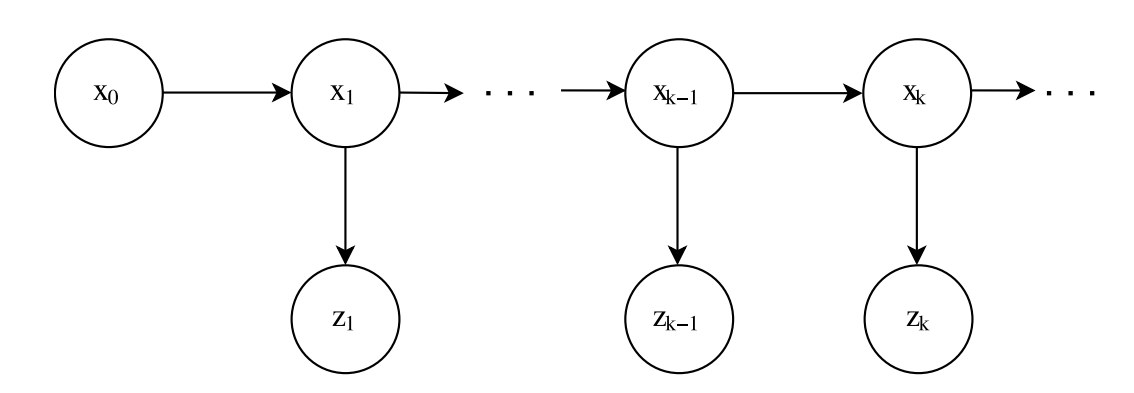
\includegraphics[width=0.6\linewidth]{img/Bayesian.png}
                        \caption{Illustration of Bayesian filtering and dependencies on time and measurement updates}
                    \end{figure}
                    \subsubsection{Time Update}
                        In the time update step, the idea is to predict the state \textbf{$x_k$} given measurements up to time k - 1, and \emph{$z^{k-1}$} this is commonly done using the Chapman–Kolmogorov equation
                        \begin{align}
                            p(x_k | z^{k-1}) = \int p(x_k | x_{k-1}) p(x_{k-1} | z^{k-1}) d x_{k-1}
                        \end{align} 
                        The transition density \emph{$p(x_k | x_{k-1})$} is defined from the choice of the motion models \textbf{$x_k = f(x_{k-1}, v_{k-1})$} where \emph{$v_k$} is a random noise process included in order to handle 
                        uncertainties and model errors. Namely the time update predicts the motion of the object.
                    \subsubsection{Measurement Update}
                        The predicted state is updated with the information from the measurement at time k. The connection between the state and the measurement is given by a measurement model \emph{$z_k = h(x_k,w_k)$}, where \emph{$w_k$} is noise. 
                        The measurement model gives rise to the likelihood of the measurement \emph{$p(z_k | x_k)$}. Since the state is estimated, it is common that the state is described by its distribution. Thus, it also includes information about 
                        the uncertainty of the estimation. We denote the prediction distribution \emph{$p_{k | k-1}(x_k | z^{k-1})$} and the posterior distribution \emph{$p_{k | k}(x_k | z^{k})$}. Subscript k | k - 1 means that the variable was 
                        computed for time \emph{k} given measurement up to time \emph{k - 1}. Similarity \emph{k | k} where measurements up to time k was used. From Bayes' theorem it follows that:
                        \begin{align}
                            p_{k|k} (x_k|z^k) \propto p(z^k|x_k) p(x_k) \propto p(z_k|x_k) p_{k|k-1} (x_k|z^{k-1})
                        \end{align}
                    \subsubsection{Kalman Filter}
                        Kalman filters have a wide variety of applications. Some of the most common applications are navigation and control for vehicles, radar tracking for anti-ballistic missiles, process control, etc. \\
                        \vspace{3mm}
                        Kalman Filter is a way of recursively finding the Bayesian estimate $\hat{x_k}$ of the true state \emph{x}. Thus it is usually more accurate than filters that compute their estimates using only the current measurement. 
                        First, at time k, a prediction is made according to the Chapman–Kolmogorov equation. When a new measurement is received, an update of said prediction is calculated based on Bayes’ theorem. How much the update relies on 
                        the prediction and the new measurement is determined by the Kalman gain, which is a way to weight the two update steps against each other, depending on their respective uncertainty. It can be shown that the (linear) 
                        Kalman filter is optimal (in the sense of minimizing the mean square error) in the cases where the noise is Gaussian.
                        \begin{figure}[H]
                            \centering
                            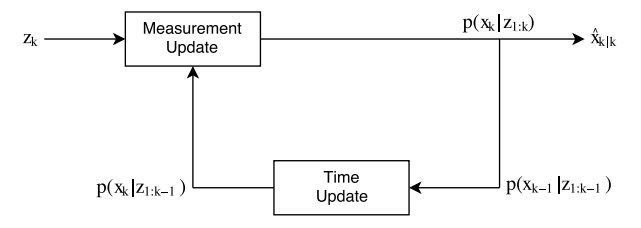
\includegraphics[width=0.6\linewidth]{img/time-measurement.png}
                            \caption{Time and measurement update}
                        \end{figure}
                            \ding{114} \textbf{Time Update} \\ 
                                \vspace{3mm}
                                As mentioned, during the time update step a prediction of the state is performed using a motion model \emph{$f(\hat{x_{k-1}}, v_{k-1})$}. In the case of linear motion 
                                \begin{align}
                                    x_k = F_{k-1} X_{k-1 | k-1} + q_{k-1}
                                \end{align}
                                The time update of the mean and covariance can be computed as 
                                \begin{align}
                                    \hat{x}_{k|k-1} = F_{k-1} \hat{x}_{k-1|k-1} \\ 
                                    P_{k|k-1} = F_{k-1} P_{k-1|k-1} F_{k-1}^T + Q_{k-1}
                                \end{align}
                                where \emph{$Q_{k-1}$} is the process noise covariance at time k-1 \\
                            \vspace{3mm}
                            \ding{114} \textbf{Measurement Update} \\ 
                                \vspace{3mm}
                                Given a new measurement \emph{$z_k$} at time \emph{k} with measurement covariance \emph{$R_k$} we can update the predicted state. In the case of linear measurement models and independent Gaussian noise, 
                                we can describe the measurement model \emph{$z_k = h(\hat{x_k}, w_k)$} as
                                \begin{align}
                                    z_k = H_k x_k + w_k
                                \end{align}  
                                The update equations of Kalman Filter are 
                                \begin{align}
                                    \hat{x}_k|k = \hat{x}_{k|k-1} + K_k v_k
                                    P_{k|k} = P_{k|k-1} - K_k S_k K_k^T
                                \end{align}
                                where the Kalman gain \emph{$K_k$} innovation \emph{$v_k$}, the innovation covariance, \emph{$S_k$} at time \emph{k} are
                                \begin{align}
                                    K_k = P_{k|k-1} H_k^T S_k^{-1}
                                    v_k = z_k - H_k \hat{x}_{k|k-1}
                                    S_k = H_k P_{k|k-1} H_k^T + R_k
                                \end{align}
                                The innovation captures the new information that the new measurement brings and the Kalman gain determines how much we should rely on this information.
                            
                    \subsubsection{Unscented Kalman Filter}
                        The Kalman filter is derived from linear models, thus is only optimal for this case and not for nonlinear models. If the models are nonlinear, linearization can be used, known as the Extended Kalman Filter (EKF). 
                        The EKF works well in many cases, although it may perform poorly if the model is significantly nonlinear within the uncertainties of the models. However, there are other methods of solving the estimation task that 
                        are more robust to nonlinearities. The derivation of the Kalman filter contains multiple integrals of the type
                        \begin{align}
                            \int g(x) \mathcal{N} (x;\hat{x};P) dx = E [g(x)]
                        \end{align}
                        where E denotes the expected value. Furthermore \emph{g(x)} is either a motion or measurement model, which can be non linear. Integrals for example in the Chapman-Kolmogorov equation may look like 
                        \begin{align}
                            \int g(x_{k-1}) \mathcal{N} (x_{k-1}; \hat{x}_{k-1|k-1}; P_{k-1|k-1}) dx_{k-1}
                        \end{align}
                        These integrals can be solved for linear models, however with nonlinear models this is not the case. Thus, these integrals needs to be approximated, one way of doing so is to use the Monte Carlo method. 
                        The idea is to generate independent and identicallyy distributed samples $x^{(1)},x^{(2)},...,x^{(N)}$ from its distribution \emph{p(x)}, that we can approximate
                        \begin{align}
                            \int g(x) p(x) dx \approx \frac{1}{N} \displaystyle\sum_{i=1}^N g(x_{(i)})
                        \end{align}
                        However as the Monte Carlo method relies on picking random samples, it might require a lot of samples in order to represent the true distribution. As an alternative, there are so called $\sigma$ -point methods which use 
                        deterministic samples chosen in clever ways to cover a large area of the space even though the number of samples is small. We will focus on one of these, the so called Unscented Kalman Filter (UKF). Two advantages of this 
                        filter are that it is efficient since it uses quite few samples, and it also only has one tuning parameter. \\ 
                        \vspace{3mm}
                            \ding{114} \textbf{Time Update} \\ 
                                \vspace{3mm}
                                With a state vector \emph{$x_k$} of dimension \emph{n}, the idea is to generate \emph{2n + 1} $\sigma$-point $\mathcal{X}$
                                \begin{align}
                                    \mathcal{X}_{k-1}^{(0)} = \hat{x}_{k-1|k-1} \\
                                    \mathcal{X}_{k-1}^{(i)} = \hat{x}_{k-1|k-1} + \sqrt{\frac{n}{1-W_0}} P_{i,k-1|k-1}^{(1/2)} & with i = 1,2,...,n \\
                                    \mathcal{X}_{k-1}^{(i+n)} = \hat{x}_{k-1|k-1} - \sqrt{\frac{n}{1-W_0}} P_{i,k-1|k-1}^{(1/2)} & with i = 1,2,...,n 
                                \end{align}
                                where \emph{$W_0$} is the tuning parameter (namely the weight of $\mathcal{X}$). \textbf{$P^{(1/2)}$} is the matrix such that
                                \begin{align}
                                    P = P^{(1/2)} (P^{(1/2)})^T
                                \end{align}
                                and \emph{$P_i^(1/2)$} is its \emph{ith} column. The UKF prediction equations are then given by
                                \begin{align}
                                    \hat{x}_{k|k-1} = \displaystyle\sum_{i=0}^{2n} f(\mathcal{X}_{k-1}^{(i)}) W_i \\
                                    P_{k|k-1} = Q_{k-1} + \displaystyle\sum_{i=0}^{2n} (f(\mathcal{X}_{k-1}^{(1)}) - \hat{x}_{k|k-1}) (.)^T W_i
                                \end{align} 
                                where $W_i = \frac{1-W_0}{2n}$ for i = 1,2,...,n. \\ 
                                \vspace{3mm}
                            \ding{114} \textbf{Measurement Update} \\ 
                            \vspace{3mm}
                                Similarly, in the measurement update step, the $\sigma$-points are chosen to 
                                \begin{align}
                                    \mathcal{X}_k^{(0)} = \hat{x}_{k|k-1} \\
                                    \mathcal{X}_k^{(i)} = \hat{x}_{k|k-1} + \sqrt{\frac{n}{1-W_0}} P_{i,k|k-1}^{(1/2)} & with i = 1,2,...,n \\
                                    \mathcal{X}_k^{i+n} = \hat{x}_{k|k-1} - \sqrt{\frac{n}{1-W_0}} P_{i,k|k-1}^{(1/2)} & with i = 1,2,...,n
                                \end{align}
                                \emph{$W_0$} is again a tuning parameter. We can now compute the necessary moments
                                \begin{align}
                                    \hat{z}_{k|k-1} = \displaystyle\sum_{i=0}^{2n} h(\chi_k^{(i)}) W_i \\ 
                                    P_{xy} = \displaystyle\sum_{i=0}^{2n} (\chi_k^{(i)} - \hat{x}_{k|k-1}) (h(\chi_k^{(i)}) - \hat{z}_{k|k-1}) \\ 
                                    S_k = R_k + \displaystyle\sum_{i=0}^{2n} (h(\chi_k^{(i)}) - \hat{z}_{k|k-1}) (.)^T W_i
                                \end{align}
                                from which the estimate and its covariance can be calculated \\ 
                                \begin{align}
                                    \hat{x}_{k|k} = \hat{x}_{k|k} + P_{xy} S_k^{-1} (z_k - \hat{z}_{k|k-1}) \\ 
                                    P_{k|k} = P_{k|k-1} - P_{xy} S_k^{-1} P_{xy}^T
                                \end{align}
                            
            \item \textbf{Deterministic Optimization} \\ 
                \vspace{3mm}
                As opposed to the probabilistic inference methods, approaches based on deterministic optimization aim to find the maximum a posteriori (MAP) solution to MOT. To that end, the task of inferring data association, the target states or both, 
                is typically cast as an optimization problem. Approaches within this framework are more suitable for the task of offline tracking because observations from all the frames or at least a time window are required to be available in advance. 
                In practice, deterministic optimization or energy minimization is employed more popularly compared with probabilistic approaches.
        \end{itemize}


\section{Detection Based Tracking Pipeline}
    \subsection{Detection Based Tracking}
        A common methodology is to split the tracking into two phases: prediction of object
        location, and matching of detections and predictions. That is, for each new frame,
        the complete tracking model does the following: \textbf{(1) Detect objects of interest, (2) Predict new locations of objects from previous frames, (3) Associate objects between frames
        by similarity of detected and predicted locations.}
    \subsection{Prediction}
        A multitude of approaches have been suggested for how to predict new locations of tracked objects. Some works include computing the optical flow to determine the new position, or using recurrent neural networks, Kalman filters or particle filters to 
        model the velocity of objects, and with this predict the position in future frames. Filtering problem is tackled in this step and methods such as Kalman filter or particle filter are among best solutions.
    \subsection{Association}
        The association task consists of determining what detection corresponds to what object, based on the predictions from the previous step, or alternatively if a detection represents a new object. Problems arise when tracked objects leave the scene or are 
        otherwise not detected, new objects enter the scene, the detector produces false positives. This step tackles assignment problems. In the case where the number of detection is equal to the number of tracked objects, this is a case of the assignment problem, 
        in which the goal is to find an optimal matching between two sets of object. Commonly, one set is called agents and the other tasks. There is a cost $c_{ij}$ associated with assigning a task j to an agent i, and the objective is to find an assignment with 
        minimum total cost, such that no agent is assigned more than one task, and no task is assigned to more than one agent. Formally, if A is the set of agents, T the set of tasks, and $x_{ij}$ represents the assignment, taking value 1 if task j is assigned to agent 
        i and 0 otherwise, then the objective is to minimize.
        \begin{align}
            \displaystyle\sum_{i \in A} \displaystyle\sum_{j \in T} c_{ij} x_{ij} \\ 
            \displaystyle]sum_{i \in A} x_{ij} = 1, j \in T \\ 
            \displaystyle\sum_{j \in T} x_{ij} = 1, i \in A \\ 
            x_{ij} \geq 0, i \in A, j \in T
        \end{align}
        One can also consider the same problem, but with the goal of maximising the cost rather
        than minimizing it.
    \subsection{Hungarian Method}
        The Hungarian algorithm, also known as Kuhn–Munkres algorithm, solves the assignment problem in polynomial time, with time complexity \emph{$O(n^3)$} where n is the number of agents (and task). The input to the algorithm is a cost matrix \emph{C}, where \emph{C(i,j)} 
        is the cost $c_{ij}$ and in four steps the matrix is manipulated to give the optimal matching. In the case where the number of agents is not equal to the number of tasks, \emph{C} can be padded with rows and columns with large values to make it square. Inversely, 
        if the goal is to find a matching with maximum cost, the matrix can be padded with zeros. Then in the final matching, assignments corresponding to added rows or columns are discarded. \\ 
        \vspace{3mm}
        Similarity measures In order to compute the cost matrix C between detections and predictions, we need to define what it means for two bounding boxes to be (dis)similar. A simple way is to compute the intersection over union (IoU), also known as the Jaccard index, between 
        two bounding boxes A and B as
        \begin{align}
            IoU(A,b) = \frac{|A \cap B|}{|A \cup B|} = \frac{|A \cap B|}{|A| + |B| - |A \cap B|} 
        \end{align}
        This has the benefit of combining distance and similarity in size and shape in a nice way, but unfortunately it gives 0 for any two bounding boxes that do not intersect. This means that if the predictions are too inaccurate, all values in the cost matrix could be 0, 
        meaning that all assignments are equally good. Despite this, IoU has successfully been used either as the only measure or in tandem with appearance information. \\ 
        \vspace{3mm}
        More sophisticated tracking models combine different similarity measures to calculate the cost, most of which can loosely be separated into three categories: distance measures, shape measures, and appearance measures. These are summed or multiplied with different weights, 
        yielding a single value indicating the overall similarity between bounding boxes. Distance and shape measures look only at the position and geometry of the bounding boxes, whereas appearance features are calculated from the actual pixels within each bounding box. \\ 
        \vspace{3mm}
        he three ingredients in the data association step including bounding box IoU, re-ID features and Kalman Filter. These are used to compute the similarity between each pair of detected boxes.We can see that only using box IoU causes a lot of ID switches. This is particularly 
        true for crowded scenes and fast camera motion. Using re-ID features alone notably increases IDF1 and decreases the number of ID switches. In addition, adding Kalman filter helps obtain smooth (reasonable) tracklets which further decreases the number of ID switches. 
        When an object is partly occluded, its re-ID features become unreliable. In this case, it is important to leverage box IoU, re-ID features and Kalman filter to obtain good tracking performance.

\section{SORT}
    \subsection{Estimation Models}
        The representation and the motion model used to propagate a target’s identity into the
        next frame.They approximate the inter-frame displacements of each object with a linear constant velocity model which is independent of other objects and camera motion. The state of
        each target is modelled as:
        \begin{align}
            x =[u,v,s,r,\dot{u},\dot{v},\dot{s}]^T
        \end{align}
        where u and v represent the horizontal and vertical pixel location of the centre of the target, while the scale s and r represent the scale (area) and the aspect ratio of the target’s bounding box respectively. Note that the aspect ratio is considered to be constant. 
        When a detection is associated to a target, the detected bounding box is used to update the target state where the velocity components are solved optimally via a Kalman filter. If no detection is associated to the target, its state is simply predicted without correction using 
        the linear velocity model.
    \subsection{Data Association}
        In assigning detections to existing targets, each target’s bounding box geometry is estimated by predicting its new location in the current frame. The assignment cost matrix is then computed as the intersection-over-union (IOU) distance between each detection and all predicted bounding boxes 
        from the existing targets. The assignment is solved optimally using the Hungarian algorithm. Additionally, a minimum IOU is imposed to reject assignments where the detection to target overlap is less than $IoU_{min}$.
    \subsection{Pipeline}
        For each frame, the following happens: objects are detected, new locations of already tracked objects are predicted using the predictors, and the detected and tracked objects are matched based on the similarities of the bounding boxes. The predictors are then updated with their associated detections, 
        and the estimated positions are returned as trackings. Additionally, new predictors are initiated for any unmatched detection, and unused predictors are removed.
        \begin{figure}[H]
            \centering
            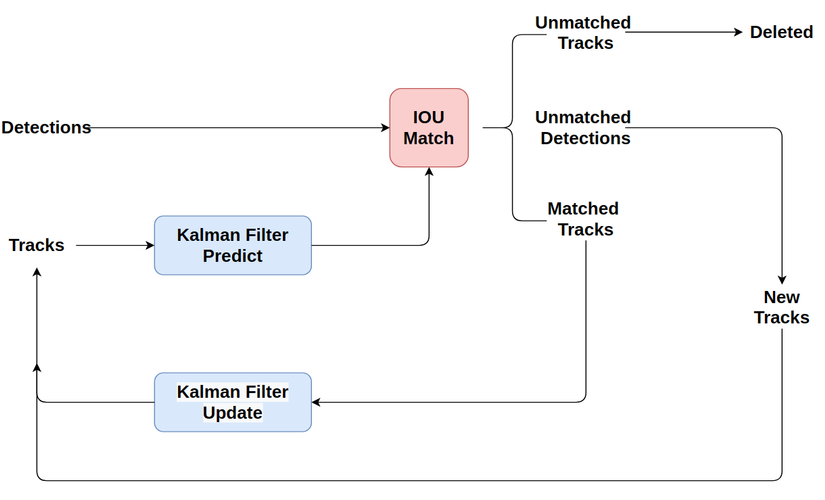
\includegraphics[width=0.6\linewidth]{img/SORT.png}
            \caption{Pipeline of SORT}
        \end{figure}
    \subsection{Pros \& Cons}
        While achieving overall good performance in terms of tracking precision and accuracy, SORT returns a relatively high number of identity switches. This is, because the employed association metric is only accurate when state estimation uncertainty is low. Therefore, SORT has a deficiency in tracking through 
        occlusions as they typically appear in frontal-view camera scenes. In addition, SORT leverage Linear Kalman Filter, which not always suits the real world application.

\section{Deep SORT}
    DeepSORT is an extension of SORT (Simple Online and Realtime Tracking), which is a simple, popular, and fast multiple-object-tracking (MOT) algorithm. DeepSORT integrates appearance information to improve the performance of SORT by adding one pretrained association metric. The core idea of DeepSORT is to use a 
    traditional single-hypothesis tracking method, which uses the Hungarian method for recursive Kalman filtering and frame-by-frame data association.
    \subsection{Improvements of DeepSORT over SORT}
        In DeepSORT, the authors solve data association problem based on Hungarian algorithm not only with IOU but also many other features: distance between detection and track, cosine distance between two feature vectors extracted from detection and track as two feature vectors of the same objects are more similar than 
        those of different objects. 
    \subsection{Data Association}
        To solve the frame-by-frame association problem, DeepSORT uses the Hungarian algorithm where both motion and appearance information are considered. This work integrate motion and appearance information through combination of two appropriate metrics. \\ 
        \vspace{3mm}
        To incorporate motion information they use the (squared) Mahalanobis distance between predicted Kalman states and newly arrived measurements:
        \begin{align}
            d^{(1)} (i,j) = (d_j - y_i)^T S_i^{-1} (d_j - y_i)
        \end{align}
        where the projection of the i-th track distribution into measurement space is denoted by ($y_i, S_i$) and the j-th bounding box detection by \emph{$d_j$}.The Mahalanobis distance takes state estimation uncertainty into account by measuring how many standard deviations the detection is away from the mean track location. 
        Further, using this metric it is possible to exclude unlikely associations by thresholding the Mahalanobis distance at a 95\% confidence interval computed from the inverse $\chi^2$ distribution. This decision is denoted by an indicator that evaluates to 1 if the association between the \emph{i-th} track and \emph{j-th} detection is admissible.
        \begin{align}
            b_{i,j}^{(1)} = \mathbb{1} [d^{(1)} (i,j) \leq t^{(1)}]
        \end{align}
        The second metric is integrated into assignment problem. For each bounding box detection $d_j$ an appearance descriptor $r_j$ is computed with $\parallel r_j \parallel = 1$. The second metric measures the smallest cosine distance between the \emph{i-th} track and \emph{j-th} detection in appearance space:
        \begin{align}
            d^{(2)} (i,j) = min\{1 - r_j^T r_k^{(1)} | r_k^{(i)} \in R_i\}
        \end{align}
        A binary variable to indicate if an association is admissible according to this metric is introduced.
        \begin{align}
            b_{i,j}^{(2)} = \mathbb{1} [d^{(2)} (i,j) \leq t^{(2)}]
        \end{align}
        In combination, both metrics complement each other by serving different aspects of the assignment problem. On the one hand, the Mahalanobis distance provides information about possible object locations based on motion that are particularly useful for short-term predictions. On the other hand, the cosine distance considers appearance information 
        that are particularly useful to recover identities after longterm occlusions, when motion is less discriminative. To build the association problem they combine both metrics using a weighted sum:
        \begin{align}
            c_{i,j} = \lambda d^{(1)} (i,j) + (1 - \lambda) d^{(2)} (i,j)
        \end{align}
        where they call an association admissible if it is within the gating region of both metrics:
        \begin{align}
            b_{i,j} = \Pi_{m = 1}^2 b_{i,j}^{(m)}
        \end{align}
        Gate matrix will be 1 only when both spatial and appearance gate functions are equal to 1 and otherwise 0 indicating whether (i, j) is a valid match for both spatial and appearance. In each new frame, the new detections are associated with existing tracks using this cost matrix and gate matrix. \\ 
        \vspace{3mm}
        The influence of each metric on the combined association cost can be controlled through hyperparameter $\lambda$.
        \begin{figure}[H]
            \centering
            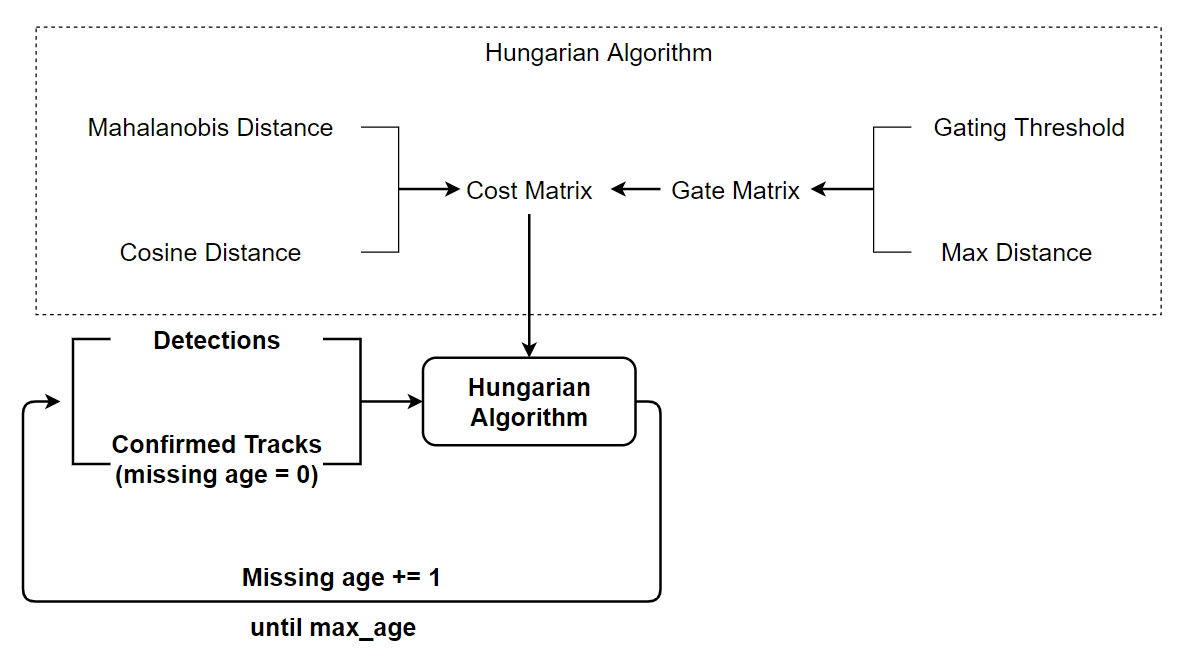
\includegraphics[width=0.6\linewidth]{img/intergrated-metrics.png}
            \caption{Data Association with two integrated metrics}
        \end{figure}
    \subsection{Deep Appearance Feature Extraction}
        The appearance information is extracted by a convolutional neural network (CNN) trained on re-identification dataset, which is Wide Residual Network. This task is also called Cosine Metric Learning. Although WRN is a shallow neural network with 16 layers, its performance is still very impressive in comparison with other thousand-layers architectures 
        with less training time and inference time.
        \begin{figure}[H]
            \centering
            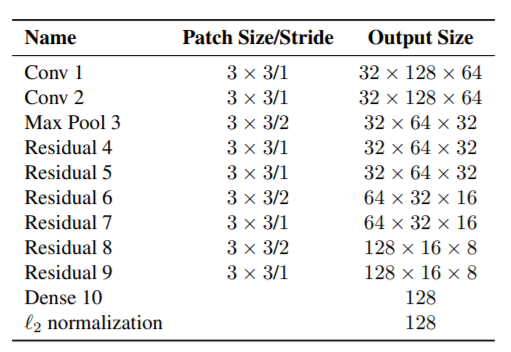
\includegraphics[width=0.6\linewidth]{img/wide-residual.png}
            \caption{Wide Residual Network Architecture}
        \end{figure}
        Consine softmax classifier is introduced and applied into training phase of this architecture
        \begin{align}
            p(y = k | \textbf{r}) = \frac{exp(\kappa . \overset{~}{\omega}_k^T \textbf{r})}{\displaystyle\sum_{n=1}^C exp(\kappa . \overset{~}{\omega}_n^T \textbf{r})}
        \end{align}
    \subsection{Matching Cascade}
        Matching Cascade recursively take track generated in the previous frame to compute cost matrix and then solve assignment problem with cascade. Below is the pseudo code of this matching stategy 
        \begin{figure}[H]
            \centering
            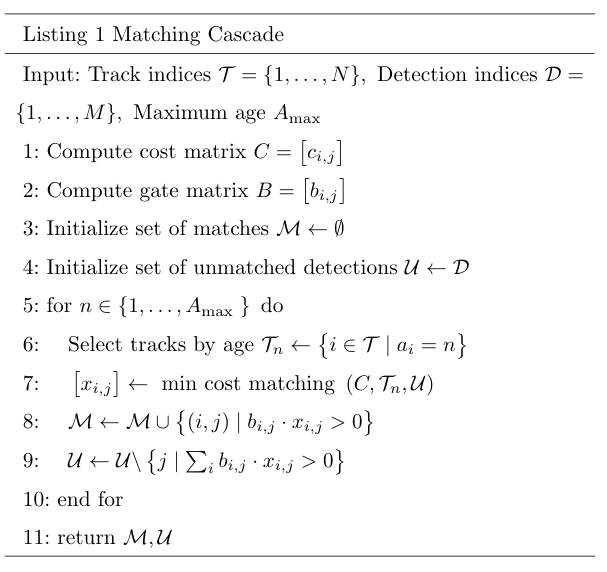
\includegraphics[width=0.6\linewidth]{img/listing.png}
            \caption{Listing of Matching Cascade}
        \end{figure}
    \subsection{Track Life Cycle Management}
        Every time a new detection is successfully associated with an existing track, the detection is added to the track and the unassociated age of the track is zero. When new detections fail to associate with existing tracks in frame f, the new detections are initialized as Tentative tracks. The original Deep SORT algorithm checks that the Tentative tracks are 
        associated with new detections in each of the \emph{$(f + 1), (f + 2),...,(f + t_{tentative})$} frames. If successfully associated, the track is updated as a Confirmed track. Otherwise, the Tentative track is deleted immediately. As for the existing tracks that fail to associate with new detections in each frame, their unassociated ages will increase by one. 
        If the unassociated age exceeds the max age threshold, the track will also be deleted.
        \begin{figure}[H]
            \centering
            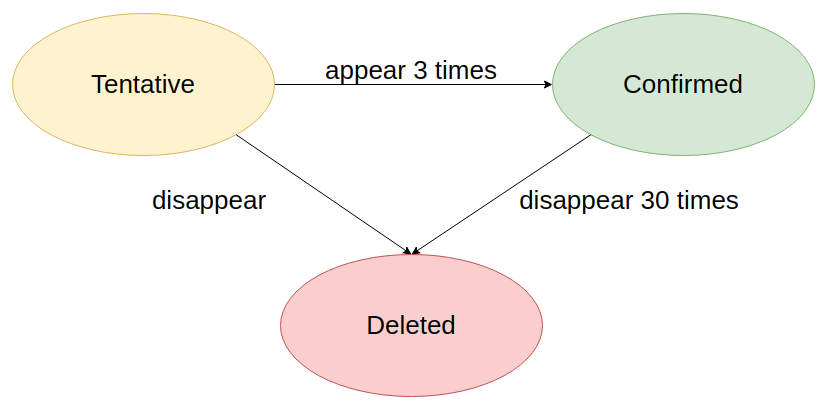
\includegraphics[width=0.6\linewidth]{img/track-life.png}
            \caption{Track Life Cycle Management}
        \end{figure}
    \subsection{Pipeline of DeepSORT}
        \begin{figure}[H]
            \centering
            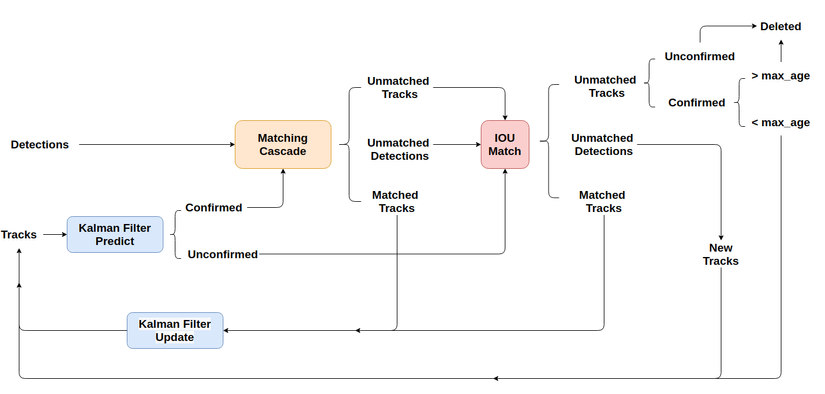
\includegraphics[width=0.6\linewidth]{img/DeepSort.png}
            \caption{Pipeline of DeepSORT}
        \end{figure}
        \begin{itemize}
            \item Firstly, Object Detection Algorithm is used to detect objects in current frame.
            \item Next, DeepSORT applies Kalman Filter to make prediction of new state base on previous state. This state is assigned with tentative value when initalized. If the value remains in the next 3 frame, the state is changed to confirmed state and will be monitoring in the next 30 frame. Otherwise, the state is released from monitoring.
            \item Using confirmed track, matching cascade is applied in order to link track with detection results based on distance metrics and appearance metrics.
            \item Tracks and detections not yet associated will go through next filter layer. Here Hungarian algorithm is used to solve assignment problem with IOU cost matrix.
            \item Classify detections and tracks prediction.
            \item Apply Kalman Filter to modify track value from associated detection and initialized new track.
        \end{itemize}

\section{Evaluations Metrics}
    \subsection{Multiple Object Tracking Accuracy(MOTA)}
        \begin{align}
            [MOTA = 1 - \frac{\sum_{t} (m_t + fp_t + mme_t)}{\sum_{t} g_t}] where (m_t, fp_t, mme_t)
        \end{align} 
        are  the number of misses, of false positives and of mismatches respectively for time t. The MOTA can be seen as composed of 3 error ratios.
        \begin{align}
            \bar{m} = \frac{\sum_{t} m_t}{\sum_{t} g_t}
        \end{align}
        the ratio of misses in the sequence, computed over the total number of objects present in all frames,
        \begin{align}
            \bar{fp} = \frac{\sum_{t} fp_t}{\sum_{t} g_t}
        \end{align}
        the ratio of false positives, and
        \begin{align}
            \bar{mme} = \frac{\sum_{t} mme_t}{\sum_{t} g_t}
        \end{align}
        the ratio of mismatches. Summing up over the different error ratios gives us the total error rate $(E_{tot})$, and $(1 - E_{tot})$ is the resulting tracking accuracy. The MOTA accounts for all object configuration errors made by the tracker, false positives, misses, mismatches, over all frames. It is similar to metrics widely used in other domains (such as the Word Error Rate (WER), 
        commonly used in speech recognition) and gives a very intuitive measure of the tracker’s performance at keeping accurate trajectories, independent of its precision in estimating object positions.
    \subsection{Multiple Object Tracking Precision(MOTP)}
        The Multiple Object Tracking Precision is the average dissimilarity between all true positives and their corresponding ground truth targets. For bounding box overlap, this is computed as
        \begin{align}
            MOTP = \frac{\sum_{t, i} d_{t, i}}{\sum_{t} c_t}
        \end{align}
        where ct denotes the number of matches in frame t and $(d_{t, i})$ is the bounding box overlap of target i with its assigned ground truth object. MOTP thereby gives the average overlap between all correctly matched hypotheses and their respective objects and ranges between \( td = 50\% \: and \: 100\% \). It is important to point out that MOTP is a measure of localization precision, 
        not to be confused with the positive predictive value or relevance in the context of precision / recall curves used, e.g., in object detection. In practice, it mostly quantifies the localization accuracy of the detector, and therefore, it provides little information about the actual performance of the tracker.
    \subsection{Average multi object tracking accuracy(AMOTA)}
        For the traditional MOTA formulation at recall \(10\%\) there are at least \(90\%\) false negatives, which may lead to negative MOTAs. Therefore the contribution of identity switches and false positives becomes negligible at low recall values. In MOTAR we include recall-normalization term \emph{\(- (1-r) * P\)} in the nominator, the factor r in the denominator and the maximum. 
        These guarantee that the values span the entire [0,1] range and brings the three error types into a similar value range. P refers to the number of ground-truth positives for the current class.
        \begin{align}
            AMOTA = \frac{1}{n - 1} \sum_{r \in {\frac{1}{n - 1}, \frac{2}{n - 1} ... 1}} MOTAR \\ 
            MOTAR = \max(0, 1 - \frac{IDS_r + FP_r + FN_r - (1 - r) * P}{r*P})
        \end{align}
    \subsection{Average multi object tracking precision(AMOTP)}
        Here ($d_{i,t}$) indicates the position error of track i at time t and ($TP_t$) indicates the number of matches at time t.
        \begin{align}
            AMOTA = \frac{1}{n - 1} \sum_{r \in {\frac{1}{n - 1}, \frac{2}{n - 1} ... 1}}\frac{\sum_{i, t} d_{i, t}}{\sum_{t} TP_t}
        \end{align}
    \subsection{Identification precision(IDP), Identification recall(IDR), IDF1}
        We use the IDFN, IDFP, IDTP counts to compute identification precision (IDP), identification recall (IDR), and the corresponding F1 score IDF1. More specifically,
        \begin{align}
            IDFN = \sum_{\tau \in AT} \sum_{t \in \mathcal{T}_\tau} m(\tau, \gamma_m(\tau),t,\Delta) \\ 
            IDFP = \sum_{\gamma \in AC} \sum_{t \in \mathcal{T}_\gamma} m(\tau_m(\gamma),\gamma,t,\Delta) \\ 
            IDTP = \sum_{\tau \in  AT} len(\tau) - IDFN = \sum_{\gamma \in  AC} len(\gamma) - IDFP
        \end{align}        
        The fraction of computed (ground truth) detections that are correctly identified.
        \begin{align}
            IDP = \frac{IDTP}{IDTP + IDFP}
            IDR = \frac{IDTP}{IDTP + IDFN}
        \end{align}
        IDF1 is the ratio of correctly identified detections over the average number of ground-truth and computed detections. ID precision and ID recall shed light on tracking trade-offs, while the IDF1 score allows ranking all trackers on a single scale that balances identification precision and recall through their harmonic mean.
        \begin{align}
            IDF_1 = \frac{2IDTP}{2IDTP + IDFP + IDFN}
        \end{align}
